\documentclass[11pt]{article}
\usepackage[T1]{fontenc}
\usepackage[utf8]{inputenc}
\usepackage{lmodern}
\usepackage[a4paper,margin=1in]{geometry}
\usepackage{amsmath,amssymb,amsthm,mathtools,bm}
\usepackage{graphicx}
\usepackage{booktabs}
\usepackage{enumitem}
\usepackage{xcolor}
\usepackage{caption}
\usepackage{subcaption}
\usepackage{hyperref}
\usepackage[nameinlink,capitalise,noabbrev]{cleveref}
\usepackage{float}
\usepackage{setspace}
\usepackage{fancyhdr}
\usepackage{array}
\usepackage{multirow}
\usepackage{longtable}
\usepackage{tikz}
\usepackage{microtype}

\setstretch{1.08}
\setlength{\parskip}{0.45em}
\setlength{\parindent}{0pt}
\setlength{\headheight}{14pt}
\allowdisplaybreaks
\numberwithin{equation}{section}

\pagestyle{fancy}
\fancyhf{}
\fancyhead[L]{Diffusion on AR(1) sequences}
\fancyhead[R]{\thepage}
\renewcommand{\headrulewidth}{0.4pt}

\newtheorem{theorem}{Theorem}[section]
\newtheorem{proposition}[theorem]{Proposition}
\newtheorem{lemma}[theorem]{Lemma}
\newtheorem{corollary}[theorem]{Corollary}
\theoremstyle{definition}
\newtheorem{definition}[theorem]{Definition}
\newtheorem{example}[theorem]{Example}
\theoremstyle{remark}
\newtheorem{remark}[theorem]{Remark}

\newcommand{\R}{\mathbb{R}}
\newcommand{\E}{\mathbb{E}}
\newcommand{\Var}{\operatorname{Var}}
\newcommand{\Cov}{\operatorname{Cov}}
\newcommand{\diag}{\operatorname{diag}}
\newcommand{\Id}{I}
\newcommand{\trans}{\mathsf{T}}
\newcommand{\diff}{\,\mathrm{d}}
\newcommand{\Ncal}{\mathcal{N}}
\newcommand{\norm}[1]{\lVert #1\rVert}
\newcommand{\inner}[2]{\langle #1,#2\rangle}
\newcommand{\argmax}{\operatorname*{arg\,max}}
\newcommand{\argmin}{\operatorname*{arg\,min}}
\newcommand{\Corr}{\operatorname{Corr}}
\newcommand{\tr}{\operatorname{tr}}
\newcommand{\sgn}{\operatorname{sgn}}


\hypersetup{
  colorlinks=true,
  linkcolor=blue!55!black,
  citecolor=blue!55!black,
  urlcolor=blue!55!black,
  pdftitle={Research continuation on diffusion over correlated sequences},
  pdfauthor={OpenAI synthesis manuscript}
}

\title{\textbf{Research Continuation on Diffusion over Correlated Sequences:}\\
Precision Lifecycle, Deterministic Limit, Fourier-Side Non-Gaussian Extensions, and Locality Observables}
\author{Structured continuation note aligned with the current manuscript}
\date{March 2026}

\begin{document}
\maketitle
\thispagestyle{empty}

\begin{abstract}
This note continues the current Gaussian AR(1) manuscript in the precise direction discussed in the meeting with Marc M\'ezard and Jerome Garnier-Brun. The benchmark case is already solved: for a Gaussian AR(1) clean trajectory observed through coordinate-wise Ornstein--Uhlenbeck noising, the noisy law remains Gaussian, the covariance evolves as $\Sigma_t=e^{-2t}\Sigma_0+\Delta_t\Id$, the score is affine, and the eigenbasis of $\Sigma_0$ exactly diagonalizes the full problem. The present note isolates what in that benchmark is specifically Gaussian, what is genuinely Markovian, and what the next structural question is.

The first main result is a sharpened analysis of the covariance--precision lifecycle. Covariance and precision respond to diffusion in fundamentally different ways. The covariance keeps the same off-diagonal profile and only contracts by the scalar factor $e^{-2t}$; the precision instead undergoes a nontrivial structural deformation: it is tridiagonal at $t=0$, becomes generically full for $t>0$, and returns to the identity in the large-time regime. We make this precise through a small-time resolvent expansion, a large-time asymptotic expansion, exact spectral formulas, and explicit locality diagnostics. The second main result is the deterministic benchmark: when the propagation is deterministic and only the initial condition is random, the clean covariance is rank one and the noisy precision is a diagonal-minus-rank-one matrix. Hence global couplings can arise even without innovation randomness; this sharply separates propagation effects from the local conditional geometry generated by genuine Markov noise. The third main result is an exact Fourier-side formulation for non-Gaussian Markov kernels of the form $M(a_{k+1}\mid a_k)\propto f(a_{k+1}-\alpha a_k)$, which gives a concrete route toward the first non-Gaussian extension. The note ends with precise locality observables, an architecture for the short and long documents, and explicit conjectures for the next mathematical and numerical steps.
\end{abstract}

\newpage
\tableofcontents
\newpage

\section{Exact statement of the open problem}

\subsection{What is already solved}

The current manuscript has established the full Gaussian AR(1) benchmark. The clean process is
\begin{equation}
 a_{k+1}=\alpha a_k+\eta_k,
 \qquad |\alpha|<1,
 \qquad \eta_k\stackrel{\mathrm{i.i.d.}}{\sim}\Ncal(0,\sigma_\eta^2),
\end{equation}
with Gaussian initial condition $a_0\sim\Ncal(\mu_0,\sigma_0^2)$, and the noised observations are
\begin{equation}
 x_k=e^{-t}a_k+\sqrt{\Delta_t}\,z_k,
 \qquad \Delta_t=1-e^{-2t},
 \qquad z_k\stackrel{\mathrm{i.i.d.}}{\sim}\Ncal(0,1).
\end{equation}
For the trajectory vectors $\mathbf a=(a_0,\dots,a_K)^\trans$ and $\mathbf x=(x_0,\dots,x_K)^\trans$, the established facts are:
\begin{align}
 \mathbf a &\sim \Ncal(\boldsymbol\mu_0,\Sigma_0), \\
 \mathbf x_t\mid \mathbf a &\sim \Ncal(e^{-t}\mathbf a,\Delta_t\Id), \\
 \mathbf x_t &\sim \Ncal(\boldsymbol\mu_t,\Sigma_t),
 \qquad \boldsymbol\mu_t=e^{-t}\boldsymbol\mu_0,
 \qquad \Sigma_t=e^{-2t}\Sigma_0+\Delta_t\Id,
\end{align}
and therefore the score is affine:
\begin{equation}\label{eq:intro_score_affine}
 S(\mathbf x,t):=\nabla_{\mathbf x}\log p_t(\mathbf x)
 =-\Sigma_t^{-1}(\mathbf x-\boldsymbol\mu_t).
\end{equation}
The current manuscript also established that the clean precision matrix $Q_0:=\Sigma_0^{-1}$ is tridiagonal, while in the eigenbasis of $\Sigma_0$ the whole Gaussian problem decouples exactly \cite{draftar1,structure,anatomy,companion}.

\subsection{What is specifically Gaussian and what is genuinely Markovian}

The Gaussian benchmark contains two distinct structural ingredients.

\begin{definition}[Gaussian ingredient]
The \emph{Gaussian ingredient} is the statement that the full law is encoded by first and second moments only. In the benchmark this yields the exact affine score \eqref{eq:intro_score_affine}, the exact spectral diagonalization of the noisy covariance, and the reduction of every structural question to the matrix $Q_t:=\Sigma_t^{-1}$.
\end{definition}

\begin{definition}[Markovian ingredient]
The \emph{Markovian ingredient} is the local factorization of the clean path measure,
\begin{equation}
 p_0(\mathbf a)=p_0(a_0)\prod_{k=0}^{K-1} M(a_{k+1}\mid a_k),
\end{equation}
which for the Gaussian AR(1) kernel becomes
\begin{equation}\label{eq:gaussian_local_factorization}
 p_0(\mathbf a)
 \propto
 \exp\!\left[-\frac{(a_0-\mu_0)^2}{2\sigma_0^2}
 -\frac{1}{2\sigma_\eta^2}\sum_{k=0}^{K-1}(a_{k+1}-\alpha a_k)^2\right].
\end{equation}
The exponent in \eqref{eq:gaussian_local_factorization} is a sum of nearest-neighbor terms on the path graph. After expansion it produces a tridiagonal Hessian, hence a tridiagonal precision matrix. This tridiagonality is the algebraic encoding of the Markov property in the Gaussian benchmark.
\end{definition}

The meeting directions emphasized that these two ingredients must now be separated conceptually. Gaussianity explains why the score is a \emph{linear operator}. Markovianity explains why that linear operator is \emph{local at clean time}. Once isotropic noise is added, Gaussianity survives but exact locality does not.

\subsection{The next mathematical question}

The next question is therefore not ``how to solve the Gaussian AR(1) model again,'' but rather:
\begin{quote}
\emph{How does the local Markov structure of the clean chain appear in the score, how is it reshaped by diffusion at intermediate times, and how is it finally erased when isotropic noise dominates?}
\end{quote}
More explicitly, the continuation problem has four layers.
\begin{enumerate}[label=(\roman*),leftmargin=1.2cm]
\item In the Gaussian benchmark, determine as sharply as possible the full lifecycle of $\Sigma_t$ and especially $Q_t=\Sigma_t^{-1}$: clean local regime, immediate loss of sparsity, intermediate delocalization, and large-time return to the identity.
\item Separate the role of genuine innovation noise from the role of deterministic propagation by studying the deterministic or nearly deterministic limit.
\item Formulate at least one non-Gaussian Markov chain with an explicitly tractable Fourier transform, and derive an exact Fourier-side representation of the noised law and the score.
\item Define observables that still measure locality when the score is no longer affine and the precision matrix is no longer the full story.
\end{enumerate}
These four layers are exactly the ones emphasized in the meeting transcript \cite{meetingtranscript}.

\section{Deep Gaussian benchmark analysis}

\subsection{Clean-time structure: why the precision is tridiagonal}

At clean time the joint density is given by \eqref{eq:gaussian_local_factorization}. Expanding the quadratic form yields
\begin{align}
&\frac{(a_0-\mu_0)^2}{2\sigma_0^2}
+\frac{1}{2\sigma_\eta^2}\sum_{k=0}^{K-1}(a_{k+1}-\alpha a_k)^2 \\
&= \frac12(\mathbf a-\boldsymbol\mu_0)^\trans Q_0(\mathbf a-\boldsymbol\mu_0),
\end{align}
with the explicit tridiagonal matrix
\begin{equation}\label{eq:Q0_explicit_here}
Q_0=
\begin{pmatrix}
\sigma_0^{-2}+\alpha^2\sigma_\eta^{-2} & -\alpha\sigma_\eta^{-2} & 0 & \cdots & 0 \\
-\alpha\sigma_\eta^{-2} & (1+\alpha^2)\sigma_\eta^{-2} & -\alpha\sigma_\eta^{-2} & \ddots & \vdots \\
0 & -\alpha\sigma_\eta^{-2} & (1+\alpha^2)\sigma_\eta^{-2} & \ddots & 0 \\
\vdots & \ddots & \ddots & \ddots & -\alpha\sigma_\eta^{-2} \\
0 & \cdots & 0 & -\alpha\sigma_\eta^{-2} & \sigma_\eta^{-2}
\end{pmatrix}.
\end{equation}

\begin{proposition}[Tridiagonal precision equals conditional locality]
Let $\mathbf X\sim\Ncal(\boldsymbol\mu,\Sigma)$ with precision $Q=\Sigma^{-1}$. Then for each index $i$,
\begin{equation}
 \E[X_i\mid X_{-i}]
 =\mu_i-\frac{1}{Q_{ii}}\sum_{j\neq i}Q_{ij}(X_j-\mu_j),
 \qquad
 \Var(X_i\mid X_{-i})=Q_{ii}^{-1}.
\end{equation}
Consequently, if $Q$ is tridiagonal then $X_i$ depends conditionally only on $X_{i-1}$ and $X_{i+1}$.
\end{proposition}

\begin{proof}
This is the standard Gaussian conditional-mean formula written in precision form. Since for \eqref{eq:Q0_explicit_here} one has $Q_{ij}=0$ whenever $|i-j|>1$, the conditional mean of the $i$-th frame depends only on its nearest neighbors. This is exactly the Markov property rewritten in Gaussian algebra.
\end{proof}

The important conceptual point is that the covariance matrix is \emph{not} local at clean time. It is dense because correlations propagate through repeated use of the recursion. The precision is local because conditioning removes indirect paths and retains only direct couplings.

\subsection{Covariance under diffusion: contraction without structural reshaping}

The noisy covariance is
\begin{equation}
 \Sigma_t=e^{-2t}\Sigma_0+\Delta_t\Id,
 \qquad \Delta_t=1-e^{-2t}.
\end{equation}
This formula has a very strong consequence.

\begin{proposition}[Covariance profile is preserved off the diagonal]\label{prop:cov_profile}
For every $j\neq k$,
\begin{equation}
 (\Sigma_t)_{jk}=e^{-2t}(\Sigma_0)_{jk}.
\end{equation}
In particular, diffusion does not create new off-diagonal covariance patterns: it only multiplies the entire off-diagonal part by the scalar factor $e^{-2t}$.
\end{proposition}

\begin{proof}
Since $\Delta_t\Id$ contributes only to the diagonal entries,
\begin{equation}
 (\Sigma_t)_{jk}=e^{-2t}(\Sigma_0)_{jk}+\Delta_t\delta_{jk}.
\end{equation}
For $j\neq k$ the Kronecker symbol vanishes and the claim follows.
\end{proof}

This is the first major separation between covariance and precision. Covariance measures \emph{marginal} correlations, and under isotropic OU noising those correlations are simply attenuated. There is no intermediate structural reorganization. The precision matrix behaves very differently because it involves a matrix inverse.

\subsection{Spectral and signal-to-noise representations of the precision}

Let
\begin{equation}
 \Sigma_0=U\Lambda U^\trans,
 \qquad
 \Lambda=\diag(\lambda_1,\dots,\lambda_N),
 \qquad \lambda_i>0.
\end{equation}
Then
\begin{equation}\label{eq:Qt_spectral_again}
Q_t:=\Sigma_t^{-1}
=U\diag\!\left(\frac{1}{e^{-2t}\lambda_i+\Delta_t}\right)U^\trans.
\end{equation}
Equivalently, with
\begin{equation}
 \gamma_t:=\frac{e^{-2t}}{\Delta_t},
\end{equation}
one has
\begin{equation}\label{eq:Qt_snr_again}
Q_t=\frac{1}{\Delta_t}(\Id+\gamma_t\Sigma_0)^{-1}.
\end{equation}

The representation \eqref{eq:Qt_spectral_again} makes the Gaussian decoupling exact in the eigenbasis. The representation \eqref{eq:Qt_snr_again} makes the original frame-basis geometry more transparent: at small time $\gamma_t\gg 1$ and signal dominates; at large time $\gamma_t\ll 1$ and isotropic noise dominates.

\subsection{Why sparsity is lost for $t>0$: algebraic and conceptual explanations}

\paragraph{Algebraic reason.}
At $t=0$, the special weights $1/\lambda_i$ in the spectral decomposition combine to reconstruct the tridiagonal inverse $Q_0$. For $t>0$, the weights become
\begin{equation}
 w_i(t)=\frac{1}{e^{-2t}\lambda_i+\Delta_t},
\end{equation}
which are no longer the clean inverse weights. Hence the cancellations required to produce tridiagonality are generically destroyed. The matrix becomes a new analytic function of $\Sigma_0$, not the exact inverse of $\Sigma_0$ itself.

\paragraph{Conceptual reason.}
At clean time the conditional dependence graph is the path graph because the path measure is a product of nearest-neighbor transition factors. After OU noising, one does not condition on the clean path itself but on a blurred observation of every coordinate. Inference about one clean coordinate therefore starts to use indirect information carried through all other noisy coordinates. The matrix $Q_t$ encodes the optimal linear denoising operator in the Gaussian benchmark; once the observations are blurred, that operator is no longer strictly local.

\subsection{Small-time expansion and immediate band fill-in}

The meeting asked whether the noisy precision becomes \emph{exactly} full immediately or merely \emph{effectively} wider. The right answer is: for generic AR(1) parameters it becomes exactly full for arbitrarily small positive times, and the widening occurs band by band with explicitly controlled small-time order.

\begin{proposition}[Resolvent expansion around $t=0$]\label{prop:resolvent_expansion}
Set
\begin{equation}
 c_t:=e^{2t}-1.
\end{equation}
Then
\begin{equation}\label{eq:Qt_resolvent_expansion}
Q_t=e^{2t}Q_0(\Id+c_tQ_0)^{-1}
=e^{2t}\sum_{m=0}^{\infty}(-c_t)^m Q_0^{m+1},
\end{equation}
whenever the Neumann series converges.
\end{proposition}

\begin{proof}
Since $\Sigma_t=e^{-2t}\Sigma_0+\Delta_t\Id$, one can factor out $e^{-2t}$ and write
\begin{equation}
 \Sigma_t=e^{-2t}(\Sigma_0+c_t\Id),
 \qquad c_t=e^{2t}-1.
\end{equation}
Hence
\begin{equation}
Q_t=e^{2t}(\Sigma_0+c_t\Id)^{-1}
=e^{2t}Q_0(\Id+c_tQ_0)^{-1}.
\end{equation}
If $\norm{c_tQ_0}<1$, the inverse is given by the convergent Neumann series
\begin{equation}
 (\Id+c_tQ_0)^{-1}=\sum_{m=0}^{\infty}(-c_t)^mQ_0^m,
\end{equation}
which yields \eqref{eq:Qt_resolvent_expansion}.
\end{proof}

\begin{theorem}[Distance-$d$ entries appear at order $t^{d-1}$]\label{thm:distance_d_order}
Let $d=|i-j|$. For $d=0$ or $d=1$, the entries of $Q_t$ are already nonzero at $t=0$. For every $d\geq 2$,
\begin{equation}\label{eq:distance_d_asymptotic}
 (Q_t)_{ij}=(-1)^{d-1}(2t)^{d-1}(Q_0^d)_{ij}+O(t^d)
 \qquad (t\downarrow 0).
\end{equation}
Moreover, $(Q_0^d)_{ij}\neq 0$ whenever $|i-j|=d$. Hence every distance class appears immediately for arbitrarily small positive times.
\end{theorem}

\begin{proof}
In \eqref{eq:Qt_resolvent_expansion}, the matrix $Q_0^{m+1}$ has bandwidth at most $m+1$ because $Q_0$ is tridiagonal. Therefore the first term that can contribute to an entry at distance $d$ is the term with $m=d-1$, namely $(-c_t)^{d-1}Q_0^d$. Since $c_t=2t+O(t^2)$, this gives \eqref{eq:distance_d_asymptotic}.

It remains to show $(Q_0^d)_{ij}\neq 0$ when $|i-j|=d$. Because $Q_0$ is tridiagonal, going from index $i$ to index $j$ in exactly $d$ matrix multiplications requires moving one step toward $j$ at each multiplication. There is therefore a unique shortest path, and its contribution is the product of the $d$ off-diagonal entries,
\begin{equation}
 (Q_0^d)_{ij}=\left(-\frac{\alpha}{\sigma_\eta^2}\right)^d,
\end{equation}
up to the obvious boundary truncations, which are still nonzero as soon as $\alpha\neq 0$. Thus the leading coefficient is nonzero.
\end{proof}

Theorem \ref{thm:distance_d_order} is the precise mathematical form of the meeting intuition: the precision matrix fills in \emph{band by band}. Distance $2$ entries appear at order $t$, distance $3$ entries at order $t^2$, and in general distance $d$ entries at order $t^{d-1}$. So the matrix is already exact-full for generic parameters as soon as $t>0$, but the farther interactions are initially extremely small.

\subsection{Large-time regime: return to isotropic noise}

The opposite regime is equally transparent.

\begin{proposition}[Large-time asymptotics]\label{prop:large_time}
As $t\to\infty$,
\begin{align}
 \Sigma_t &= \Id+e^{-2t}(\Sigma_0-\Id), \\
 Q_t &= \Id-e^{-2t}(\Sigma_0-\Id)+O(e^{-4t}).
\end{align}
In particular, for $i\neq j$,
\begin{equation}
 (Q_t)_{ij}=-e^{-2t}(\Sigma_0)_{ij}+O(e^{-4t}),
\end{equation}
so every off-diagonal coupling decays exponentially to zero.
\end{proposition}

\begin{proof}
The formula for $\Sigma_t$ is immediate from $\Delta_t=1-e^{-2t}$. Then
\begin{equation}
 Q_t=(\Id+e^{-2t}(\Sigma_0-\Id))^{-1},
\end{equation}
and the claim follows from the resolvent identity $(\Id+B)^{-1}=\Id-B+O(\norm{B}^2)$ with $B=e^{-2t}(\Sigma_0-\Id)$.
\end{proof}

This proves precisely why the end of diffusion ``kills the Markov structure.'' It does not return to the clean path graph. It returns to the diagonal identity matrix because the law becomes dominated by independent isotropic Gaussian noise.

\subsection{Conditioning and modewise flattening}

The eigenvalues of $\Sigma_t$ are
\begin{equation}
 \lambda_i(t)=e^{-2t}\lambda_i+(1-e^{-2t})=1+e^{-2t}(\lambda_i-1),
\end{equation}
while the eigenvalues of $Q_t$ are $\lambda_i(t)^{-1}$. Hence
\begin{equation}\label{eq:kappa_formula}
 \kappa(\Sigma_t)
 =\frac{1+e^{-2t}(\lambda_{\max}-1)}{1+e^{-2t}(\lambda_{\min}-1)}.
\end{equation}

\begin{proposition}[Condition number decreases monotonically]
The function $t\mapsto \kappa(\Sigma_t)$ is nonincreasing and converges to $1$ as $t\to\infty$.
\end{proposition}

\begin{proof}
Write $s=e^{-2t}\in(0,1]$. Then
\begin{equation}
 \kappa(\Sigma_t)=\frac{1+s(\lambda_{\max}-1)}{1+s(\lambda_{\min}-1)}.
\end{equation}
Differentiating with respect to $s$ gives
\begin{equation}
 \frac{\diff}{\diff s}\kappa
 =\frac{\lambda_{\max}-\lambda_{\min}}{(1+s(\lambda_{\min}-1))^2}\geq 0.
\end{equation}
Since $s'(t)=-2e^{-2t}<0$, the derivative with respect to $t$ is nonpositive. The limit $t\to\infty$ corresponds to $s\to 0$, which gives $\kappa\to 1$.
\end{proof}

Thus diffusion has two simultaneous effects: it destroys exact locality in the frame basis, but it improves conditioning and simplifies the problem in spectral coordinates. The intermediate regime is therefore the genuinely interesting one.

\subsection{Intermediate regime and quantitative diagnostics}

To study the intermediate regime one needs diagnostics that go beyond visual heatmaps.

\begin{definition}[Band projection and band mass]
For any matrix $A\in\R^{N\times N}$ and radius $r\in\{0,1,\dots,N-1\}$, define the band projection
\begin{equation}
 (\mathcal B_rA)_{ij}:=A_{ij}\mathbf 1_{\{|i-j|\leq r\}}.
\end{equation}
Define the entrywise band mass fraction by
\begin{equation}
 T_r(A):=\frac{\sum_{|i-j|\leq r}|A_{ij}|}{\sum_{i,j}|A_{ij}|}
 =\frac{\|\mathcal B_rA\|_{1,\mathrm{entry}}}{\|A\|_{1,\mathrm{entry}}}.
\end{equation}
For the precision matrix we write $T_r(t):=T_r(Q_t)$.
\end{definition}

The tridiagonal mass fraction $T_1(t)$ is the most direct scalar summary of ``how Markovian'' the Gaussian score still looks in the original frame basis.

\begin{definition}[Off-band mass and effective bandwidth]
For $r\geq 0$ define the off-band mass
\begin{equation}
 O_r(t):=1-T_r(t).
\end{equation}
Given a target mass level $\rho\in(0,1)$, define the effective bandwidth
\begin{equation}
 b_\rho(t):=\min\{r:\ T_r(t)\geq \rho\}.
\end{equation}
\end{definition}

\begin{definition}[Row interaction range]
For row $k$, define the weight profile $w_{kj}(t):=|Q_t(k,j)|$ and the row interaction range
\begin{equation}
 \xi_k(t):=\frac{\sum_j |j-k|w_{kj}(t)}{\sum_j w_{kj}(t)}.
\end{equation}
The average interaction range is
\begin{equation}
 \bar\xi(t):=\frac{1}{N}\sum_{k=0}^{N-1}\xi_k(t).
\end{equation}
\end{definition}

\begin{proposition}[Existence of a maximally delocalized time]
For each fixed band radius $r$, the function $O_r(t)$ is continuous for $t>0$ and satisfies
\begin{equation}
 \lim_{t\downarrow 0}O_r(t)=0,
 \qquad
 \lim_{t\to\infty}O_r(t)=0.
\end{equation}
Hence $O_r$ attains at least one maximum at an intermediate time $t_r^*\in(0,\infty)$.
The same is true for any continuous delocalization observable such as $\bar\xi(t)$.
\end{proposition}

\begin{proof}
Continuity follows because $Q_t$ depends smoothly on $t$ for $t>0$. The small-time limit is zero because $Q_t\to Q_0$ and $Q_0$ is tridiagonal. The large-time limit is zero because $Q_t\to\Id$, which is diagonal. A continuous function that vanishes at both ends of the interval must attain its maximum at an interior point.
\end{proof}

Numerically, with the stationary benchmark parameters used in the figures, the average interaction range is maximal near $t\approx 1.21$ while the tridiagonal mass fraction is minimal near $t\approx 0.76$. These times need not coincide because they measure different aspects of delocalization. One measures global band mass, the other the average rowwise spread.

\subsection{Neighboring score components and the posterior-mean viewpoint}

The meeting emphasized two related objects: the relation between neighboring score components and the conditional mean $\E[\mathbf a\mid \mathbf x_t=\mathbf x]$.

\begin{proposition}[Score covariance equals precision]\label{prop:score_cov}
In the Gaussian benchmark,
\begin{equation}
 S_t:=-Q_t(\mathbf X_t-\boldsymbol\mu_t)
\end{equation}
satisfies
\begin{equation}
 \Cov(S_t)=Q_t.
\end{equation}
Hence the covariance and correlation of the score components are exactly controlled by the noisy precision matrix.
\end{proposition}

\begin{proof}
Using symmetry of $Q_t$,
\begin{equation}
 \Cov(S_t)=Q_t\Sigma_tQ_t=Q_t.
\end{equation}
\end{proof}

This is important because it answers the meeting question on $S_k$ versus $S_{k+1}$ at fixed diffusion time. In the Gaussian benchmark,
\begin{equation}
 \Cov(S_k,S_{k+1})=(Q_t)_{k,k+1},
 \qquad
 \Corr(S_k,S_{k+1})=\frac{(Q_t)_{k,k+1}}{\sqrt{(Q_t)_{kk}(Q_t)_{k+1,k+1}}}.
\end{equation}
Thus neighboring-score dependence is not an additional object: it is a normalized slice of the precision matrix itself.

Now turn to the posterior mean. For the OU observation model,
\begin{equation}
 \mathbf X_t=e^{-t}\mathbf a+\sqrt{\Delta_t}\,\mathbf Z,
\end{equation}
there is a vector-valued Tweedie formula.

\begin{proposition}[Posterior mean identity]\label{prop:tweedie_vector}
For any prior law on $\mathbf a$ with finite first moment,
\begin{equation}\label{eq:tweedie_vector}
 \E[\mathbf a\mid \mathbf X_t=\mathbf x]
 =e^t\big(\mathbf x+\Delta_t\nabla_{\mathbf x}\log p_t(\mathbf x)\big).
\end{equation}
In the Gaussian benchmark this becomes
\begin{equation}\label{eq:posterior_mean_gaussian}
 \E[\mathbf a\mid \mathbf X_t=\mathbf x]
 =\boldsymbol\mu_0+e^{-t}\Sigma_0Q_t(\mathbf x-\boldsymbol\mu_t).
\end{equation}
\end{proposition}

\begin{proof}
The identity \eqref{eq:tweedie_vector} is the standard Gaussian-channel posterior mean formula. In the Gaussian benchmark, substitute $\nabla\log p_t(\mathbf x)=-Q_t(\mathbf x-\boldsymbol\mu_t)$ and use $\Sigma_t=e^{-2t}\Sigma_0+\Delta_t\Id$ to obtain
\begin{equation}
 e^t\big(\mathbf x-\Delta_tQ_t(\mathbf x-\boldsymbol\mu_t)\big)
 =\boldsymbol\mu_0+e^{-t}\Sigma_0Q_t(\mathbf x-\boldsymbol\mu_t).
\end{equation}
\end{proof}

The matrix
\begin{equation}\label{eq:gain_matrix_def}
 G_t:=e^{-t}\Sigma_0Q_t
 =e^t(\Id-\Delta_tQ_t)
\end{equation}
is the linear gain from the observation $\mathbf x$ to the posterior mean. It is often more intuitive than $Q_t$ because it tells us directly which coordinates of $\mathbf x$ are used to reconstruct a given clean frame. At small time $G_t\to \Id$, so one mostly uses the corresponding coordinate. At large time $G_t\to 0$, so the posterior mean collapses to the prior mean and no coordinate matters any longer.

\section{Deterministic and nearly deterministic limits}

\subsection{Pure deterministic propagation with random initial condition}

The clean stochastic AR(1) process mixes two sources of uncertainty: the random initial condition and the innovation sequence. To isolate propagation effects, consider the deterministic propagation model
\begin{equation}\label{eq:det_model}
 a_k=\alpha^kA_0,
 \qquad A_0\sim\Ncal(\mu_0,\sigma_0^2),
 \qquad |\alpha|<1.
\end{equation}
Equivalently, the transition kernel is a Dirac mass,
\begin{equation}
 M(a_{k+1}\mid a_k)=\delta(a_{k+1}-\alpha a_k).
\end{equation}
Every randomness comes from the one-dimensional latent amplitude $A_0$.

\begin{proposition}[Clean covariance in the deterministic model]
Let
\begin{equation}
 v=(1,\alpha,\alpha^2,\dots,\alpha^K)^\trans.
\end{equation}
Then
\begin{equation}\label{eq:det_rank_one_cov}
 \mathbf a=A_0v,
 \qquad
 \boldsymbol\mu_0=\mu_0v,
 \qquad
 \Sigma_0^{\mathrm{det}}=\sigma_0^2vv^\trans.
\end{equation}
In particular, the clean covariance is rank one and therefore singular.
\end{proposition}

\begin{proof}
Since $a_k=\alpha^kA_0$, one has $\mathbf a=A_0v$. Taking mean and covariance gives the result immediately.
\end{proof}

After OU noising,
\begin{equation}
 \mathbf X_t=e^{-t}A_0v+\sqrt{\Delta_t}\,\mathbf Z,
\end{equation}
so
\begin{equation}\label{eq:det_noisy_cov}
 \Sigma_t^{\mathrm{det}}=
 e^{-2t}\sigma_0^2vv^\trans+\Delta_t\Id.
\end{equation}
Because \eqref{eq:det_noisy_cov} is a diagonal matrix plus a rank-one perturbation, its inverse is explicit.

\begin{proposition}[Exact noisy precision in the deterministic benchmark]\label{prop:det_precision}
For every $t>0$,
\begin{equation}\label{eq:det_precision_formula}
 Q_t^{\mathrm{det}}
 :=(\Sigma_t^{\mathrm{det}})^{-1}
 =\frac{1}{\Delta_t}\Id
 -\frac{e^{-2t}\sigma_0^2}{\Delta_t^2\big(1+\frac{e^{-2t}\sigma_0^2}{\Delta_t}\norm{v}^2\big)}vv^\trans.
\end{equation}
Hence for $i\neq j$,
\begin{equation}
 (Q_t^{\mathrm{det}})_{ij}
 =-\frac{e^{-2t}\sigma_0^2}{\Delta_t^2\big(1+\frac{e^{-2t}\sigma_0^2}{\Delta_t}\norm{v}^2\big)}\alpha^{i+j},
\end{equation}
which is generically nonzero for every pair $(i,j)$.
\end{proposition}

\begin{proof}
Apply the Sherman--Morrison formula to
\begin{equation}
 \Sigma_t^{\mathrm{det}}=\Delta_t\Id+c_tvv^\trans,
 \qquad c_t=e^{-2t}\sigma_0^2.
\end{equation}
Then
\begin{equation}
 (\Delta_t\Id+c_tvv^\trans)^{-1}
 =\Delta_t^{-1}\Id-\frac{c_t}{\Delta_t^2(1+\frac{c_t}{\Delta_t}v^\trans v)}vv^\trans,
\end{equation}
which is exactly \eqref{eq:det_precision_formula}.
\end{proof}

This deterministic benchmark is highly informative. In the stochastic Gaussian AR(1) model, locality at $t=0$ came from the path-graph factorization of the clean law. In the deterministic benchmark there is no such graph-local precision at all because the clean covariance is singular rank one. After noising, the inverse is immediately a diagonal-minus-rank-one dense matrix. Therefore:
\begin{quote}
\emph{Global structure in the score can be produced by deterministic propagation of a single latent variable even in the complete absence of innovation randomness.}
\end{quote}
So one must distinguish carefully between two different mechanisms for long-range effects:
\begin{enumerate}[label=(\alph*),leftmargin=1cm]
\item global couplings caused by common latent amplitude propagation, and
\item global couplings caused by diffusion destroying the exact sparse cancellation of a genuinely local Markov precision.
\end{enumerate}

\subsection{Score and posterior mean in the deterministic benchmark}

The noisy mean is $\boldsymbol\mu_t^{\mathrm{det}}=e^{-t}\mu_0v$, so the score is still affine:
\begin{equation}
 S^{\mathrm{det}}(\mathbf x,t)
 =-Q_t^{\mathrm{det}}(\mathbf x-\boldsymbol\mu_t^{\mathrm{det}}).
\end{equation}
The posterior mean can be written in scalar form because the latent uncertainty is one-dimensional.

\begin{proposition}[Posterior mean in the deterministic benchmark]
For $t>0$,
\begin{equation}\label{eq:det_scalar_posterior}
 \E[A_0\mid \mathbf X_t=\mathbf x]
 =\mu_0+
 \frac{e^{-t}\sigma_0^2}{\Delta_t+e^{-2t}\sigma_0^2\norm{v}^2}
 v^\trans(\mathbf x-\boldsymbol\mu_t^{\mathrm{det}}).
\end{equation}
Therefore
\begin{equation}
 \E[\mathbf a\mid \mathbf X_t=\mathbf x]
 =v\,\E[A_0\mid \mathbf X_t=\mathbf x].
\end{equation}
Every posterior coordinate depends on the same global sufficient statistic $v^\trans\mathbf x$.
\end{proposition}

\begin{proof}
This is one-dimensional Gaussian linear regression for the channel
\begin{equation}
 \mathbf X_t=e^{-t}A_0v+\sqrt{\Delta_t}\,\mathbf Z.
\end{equation}
The posterior precision of $A_0$ is
\begin{equation}
 \sigma_0^{-2}+\frac{e^{-2t}}{\Delta_t}\norm{v}^2,
\end{equation}
and the posterior mean is given by the usual Bayesian linear-Gaussian formula.
\end{proof}

The deterministic benchmark therefore answers Jerome's conditional-mean intuition in the clearest possible way: when the clean process is generated by a single latent scalar, the ``best reconstruction'' of any frame uses a global weighted average of all observations, not local neighbors.

\subsection{Nearly deterministic regime and noncommuting limits}

Now return to the stochastic Gaussian AR(1) process, but let the innovation variance be small. For $j\leq k$,
\begin{equation}\label{eq:cov_small_sigma_eta}
 \Cov(a_j,a_k)=\alpha^{j+k}\sigma_0^2+
 \sigma_\eta^2\,\alpha^{k-j}\frac{1-\alpha^{2j}}{1-\alpha^2}.
\end{equation}
This yields the decomposition
\begin{equation}\label{eq:cov_decomp_small_sigma}
 \Sigma_0=\sigma_0^2vv^\trans+\sigma_\eta^2 B,
\end{equation}
where
\begin{equation}
 B_{jk}=\frac{\alpha^{|j-k|}-\alpha^{j+k}}{1-\alpha^2}.
\end{equation}
Thus for fixed $t>0$,
\begin{equation}
 \Sigma_t=\Delta_t\Id+e^{-2t}\sigma_0^2vv^\trans+e^{-2t}\sigma_\eta^2B.
\end{equation}

\begin{proposition}[Small-$\sigma_\eta^2$ expansion at fixed $t>0$]\label{prop:small_sigma_eta}
Let $Q_t^{\mathrm{det}}$ be the deterministic precision \eqref{eq:det_precision_formula}. For each fixed $t>0$,
\begin{equation}\label{eq:small_sigma_eta_expansion}
 Q_t=Q_t^{\mathrm{det}}-e^{-2t}\sigma_\eta^2Q_t^{\mathrm{det}}BQ_t^{\mathrm{det}}+O(\sigma_\eta^4).
\end{equation}
\end{proposition}

\begin{proof}
Write
\begin{equation}
 \Sigma_t=\Sigma_t^{\mathrm{det}}+e^{-2t}\sigma_\eta^2B.
\end{equation}
Since $\Sigma_t^{\mathrm{det}}$ is positive definite for $t>0$, the standard resolvent expansion gives
\begin{equation}
 (A+\varepsilon B)^{-1}=A^{-1}-\varepsilon A^{-1}BA^{-1}+O(\varepsilon^2)
\end{equation}
with $A=\Sigma_t^{\mathrm{det}}$ and $\varepsilon=e^{-2t}\sigma_\eta^2$.
\end{proof}

The key lesson is that the limits $t\downarrow 0$ and $\sigma_\eta^2\downarrow 0$ do not commute.

\begin{itemize}[leftmargin=1.2cm]
\item If one fixes $\sigma_\eta^2>0$ and sends $t\downarrow 0$, one recovers the tridiagonal Markov precision $Q_0$.
\item If one first sets $\sigma_\eta^2=0$ and only then studies $t>0$, one obtains the dense rank-one-corrected inverse \eqref{eq:det_precision_formula}.
\end{itemize}
This noncommutation is mathematically important because it separates a \emph{singular clean-time Markov limit} from a \emph{regular noised deterministic limit}.

\section{Non-Gaussian candidate models and the strongest first extension}

\subsection{General Markov kernel with known Fourier transform}

Consider the non-Gaussian Markov chain
\begin{equation}\label{eq:general_non_gaussian_chain}
 a_{k+1}=\alpha a_k+\varepsilon_k,
 \qquad \varepsilon_k\stackrel{\mathrm{i.i.d.}}{\sim}f,
\end{equation}
where $f$ is a centered non-Gaussian density with known characteristic function
\begin{equation}
 \widehat f(q):=\E[e^{iq\varepsilon_0}].
\end{equation}
Let the initial condition be independent of the innovations with characteristic function
\begin{equation}
 \phi_0(q):=\E[e^{iq a_0}].
\end{equation}
The chain still has the explicit unrolled form
\begin{equation}\label{eq:unrolled_general_chain}
 a_k=\alpha^k a_0+\sum_{\ell=0}^{k-1}\alpha^{k-1-\ell}\varepsilon_\ell.
\end{equation}
This already gives the exact clean characteristic function.

\begin{theorem}[Exact characteristic function of the full clean trajectory]\label{thm:char_function_general}
Let $\xi=(\xi_0,\dots,\xi_K)^\trans\in\R^{K+1}$. Define the tail linear forms
\begin{align}
 L_0(\xi)&:=\sum_{k=0}^K\alpha^k\xi_k, \\
 L_{\ell+1}(\xi)&:=\sum_{k=\ell+1}^K\alpha^{k-1-\ell}\xi_k,
 \qquad \ell=0,1,\dots,K-1.
\end{align}
Then the characteristic function of the clean trajectory is
\begin{equation}\label{eq:general_char_clean}
 \Phi_0(\xi)
 :=\E\big[e^{i\sum_{k=0}^K\xi_ka_k}\big]
 =\phi_0\big(L_0(\xi)\big)
 \prod_{\ell=0}^{K-1}\widehat f\big(L_{\ell+1}(\xi)\big).
\end{equation}
\end{theorem}

\begin{proof}
Insert \eqref{eq:unrolled_general_chain} into $\sum_k\xi_ka_k$:
\begin{align}
 \sum_{k=0}^K\xi_ka_k
 &=a_0\sum_{k=0}^K\alpha^k\xi_k
 +\sum_{k=0}^K\xi_k\sum_{\ell=0}^{k-1}\alpha^{k-1-\ell}\varepsilon_\ell \\
 &=a_0L_0(\xi)+\sum_{\ell=0}^{K-1}\varepsilon_\ell\sum_{k=\ell+1}^K\alpha^{k-1-\ell}\xi_k \\
 &=a_0L_0(\xi)+\sum_{\ell=0}^{K-1}\varepsilon_\ell L_{\ell+1}(\xi).
\end{align}
Now use independence of $a_0$ and the innovations to factor expectations.
\end{proof}

The OU noising step preserves an equally simple Fourier representation.

\begin{proposition}[Characteristic function after OU noising]\label{prop:char_function_noisy}
Let
\begin{equation}
 \mathbf X_t=e^{-t}\mathbf a+\sqrt{\Delta_t}\,\mathbf Z,
 \qquad \mathbf Z\sim\Ncal(0,\Id),
\end{equation}
independent of $\mathbf a$. Then
\begin{equation}\label{eq:char_noisy_general}
 \Phi_t(\xi)
 :=\E[e^{i\xi^\trans\mathbf X_t}]
 =\exp\!\left(-\frac{\Delta_t}{2}\norm{\xi}^2\right)
 \Phi_0(e^{-t}\xi).
\end{equation}
Consequently,
\begin{equation}\label{eq:inverse_fourier_general}
 p_t(\mathbf x)=\frac{1}{(2\pi)^N}
 \int_{\R^N}
 e^{-i\xi^\trans\mathbf x}
 e^{-\frac{\Delta_t}{2}\norm{\xi}^2}
 \Phi_0(e^{-t}\xi)
 \,\diff\xi.
\end{equation}
\end{proposition}

\begin{proof}
Condition on $\mathbf a$ and use the characteristic function of the Gaussian noise. Then remove the conditioning.
\end{proof}

This is the exact Fourier-side continuation of the Gaussian benchmark. The Gaussian case is the special case in which $\log \widehat f$ is quadratic, so the inverse transform remains Gaussian and the score becomes affine.

\subsection{Candidate non-Gaussian models}

The natural first candidates are the following.

\begin{enumerate}[label=\textbf{C\arabic*.},leftmargin=1.2cm]
\item \textbf{Laplace innovations.}
\begin{equation}
 f(u)=\frac{1}{2b}e^{-|u|/b},
 \qquad
 \widehat f(q)=\frac{1}{1+b^2q^2}.
\end{equation}
This model has finite variance $2b^2$, a simple rational Fourier transform, and a clean small-frequency Gaussian approximation.

\item \textbf{Symmetric $\beta$-stable innovations.}
\begin{equation}
 \widehat f(q)=\exp(-c|q|^\beta),
 \qquad 0<\beta\leq 2.
\end{equation}
The case $\beta=2$ is Gaussian, while $\beta=1$ is Cauchy. The Fourier exponent is extremely simple, but the law can have infinite variance, which moves farther away from the current benchmark.

\item \textbf{Two-component Gaussian mixture innovations.}
\begin{equation}
 f(u)=w\,\Ncal(0,\sigma_1^2)+(1-w)\,\Ncal(0,\sigma_2^2),
 \qquad
 \widehat f(q)=we^{-\sigma_1^2q^2/2}+(1-w)e^{-\sigma_2^2q^2/2}.
\end{equation}
This keeps finite moments and strong numerical tractability, but the Fourier logarithm no longer linearizes as cleanly as in the Laplace or stable families.

\item \textbf{Student-type innovations as Gaussian scale mixtures.}
These are attractive for robustness but their Fourier transforms and inverse transforms are more cumbersome at the multivariate path level.
\end{enumerate}

\subsection{Why Laplace is the strongest first step}

For the first non-Gaussian extension, the Laplace kernel is the strongest candidate for three reasons.
\begin{enumerate}[label=(\arabic*),leftmargin=1cm]
\item It is truly non-Gaussian but still has finite variance, so it remains close enough to the Gaussian benchmark to make comparisons meaningful.
\item Its characteristic function is rational, hence easy to insert into \eqref{eq:general_char_clean} and \eqref{eq:char_noisy_general}.
\item Its small-frequency expansion reproduces the Gaussian benchmark with an effective innovation variance $2b^2$, so the benchmark appears as the quadratic tangent of the non-Gaussian model.
\end{enumerate}

Assume now that $a_0\sim\Ncal(\mu_0,\sigma_0^2)$ while the innovations are Laplace. Then
\begin{equation}
 \phi_0(q)=\exp\!\left(i\mu_0q-\frac{\sigma_0^2q^2}{2}\right),
 \qquad
 \widehat f(q)=\frac{1}{1+b^2q^2}.
\end{equation}
By \Cref{thm:char_function_general,prop:char_function_noisy},
\begin{equation}\label{eq:laplace_char_noisy}
 \Phi_t^{\mathrm{Lap}}(\xi)
 =\exp\!\left(-\frac{\Delta_t}{2}\norm{\xi}^2
 +ie^{-t}\mu_0L_0(\xi)
 -\frac{e^{-2t}\sigma_0^2}{2}L_0(\xi)^2\right)
 \prod_{\ell=0}^{K-1}
 \frac{1}{1+b^2e^{-2t}L_{\ell+1}(\xi)^2}.
\end{equation}
Therefore
\begin{equation}\label{eq:laplace_density_inverse}
 p_t^{\mathrm{Lap}}(\mathbf x)
 =\frac{1}{(2\pi)^N}\int_{\R^N}
 e^{-i\xi^\trans\mathbf x}\Phi_t^{\mathrm{Lap}}(\xi)
 \,\diff\xi.
\end{equation}
The score is given exactly by differentiating under the integral sign:
\begin{equation}\label{eq:laplace_score_ratio}
 S^{\mathrm{Lap}}(\mathbf x,t)
 =\frac{\int_{\R^N}(-i\xi)
 e^{-i\xi^\trans\mathbf x}\Phi_t^{\mathrm{Lap}}(\xi)
 \,\diff\xi}{\int_{\R^N}
 e^{-i\xi^\trans\mathbf x}\Phi_t^{\mathrm{Lap}}(\xi)
 \,\diff\xi}.
\end{equation}
This is not affine anymore, but it is exact.

\subsection{Gaussian benchmark as the low-frequency tangent of the Laplace model}

The small-frequency expansion of the Laplace characteristic function is
\begin{equation}
 \log\frac{1}{1+b^2q^2}
 =-b^2q^2+O(q^4),
 \qquad q\to 0.
\end{equation}
Thus
\begin{align}
 \log \Phi_t^{\mathrm{Lap}}(\xi)
 &= -\frac{\Delta_t}{2}\norm{\xi}^2
 +ie^{-t}\mu_0L_0(\xi)
 -\frac{e^{-2t}\sigma_0^2}{2}L_0(\xi)^2
 -b^2e^{-2t}\sum_{\ell=0}^{K-1}L_{\ell+1}(\xi)^2
 +O(\norm{\xi}^4).
\end{align}
Comparing with the Gaussian AR(1) exponent shows that the effective Gaussian innovation variance is
\begin{equation}
 \sigma_{\eta,\mathrm{eff}}^2=2b^2.
\end{equation}
So the current Gaussian benchmark is the quadratic low-frequency tangent of the Laplace chain. This is exactly the kind of bridge one wants for a first non-Gaussian extension.

\subsection{What replaces the precision matrix when the score is nonlinear}

In the Gaussian benchmark the constant matrix $Q_t$ entirely governs the score. In a non-Gaussian model the correct replacement is no longer a constant matrix but an \emph{$x$-dependent local operator}.

\begin{definition}[Observed precision or score Hessian]
For a smooth noisy density $p_t$, define
\begin{equation}\label{eq:observed_precision_def}
 \mathcal H_t(\mathbf x):=-\nabla_{\mathbf x}^2\log p_t(\mathbf x).
\end{equation}
In the Gaussian case, $\mathcal H_t(\mathbf x)\equiv Q_t$ is constant. In the non-Gaussian case, $\mathcal H_t(\mathbf x)$ is the pointwise Jacobian of the score and is the natural local-dependence matrix.
\end{definition}

The posterior mean still satisfies the exact identity \eqref{eq:tweedie_vector}. Therefore its Jacobian is
\begin{equation}
 \nabla_{\mathbf x}\E[\mathbf a\mid \mathbf X_t=\mathbf x]
 =e^t\big(\Id+\Delta_t\nabla_{\mathbf x}S(\mathbf x,t)\big)
 =e^t\big(\Id-\Delta_t\mathcal H_t(\mathbf x)\big).
\end{equation}
This matrix is the natural nonlinear analogue of the Gaussian gain matrix $G_t$.

\section{Locality observables for the score and the posterior mean}

The meeting requested observables that remain meaningful even when the score becomes nonlinear. The benchmark suggests a hierarchy.

\subsection{Gaussian observables}

When the score is affine, everything reduces to matrices.

\begin{definition}[Gaussian locality observables]
For the Gaussian benchmark define:
\begin{enumerate}[label=(\roman*),leftmargin=1.2cm]
\item the band-mass profile $T_r(t)$ and off-band mass $O_r(t)$ from the precision matrix $Q_t$;
\item the effective bandwidth $b_\rho(t)$;
\item the row interaction range $\xi_k(t)$ and its average $\bar\xi(t)$;
\item the neighboring-score covariance and correlation,
\begin{equation}
 \Cov(S_k,S_{k+1})=(Q_t)_{k,k+1},
 \qquad
 \Corr(S_k,S_{k+1})=\frac{(Q_t)_{k,k+1}}{\sqrt{(Q_t)_{kk}(Q_t)_{k+1,k+1}}};
\end{equation}
\item the posterior-mean sensitivity matrix $G_t=e^{-t}\Sigma_0Q_t$ and the analogous observables built from $|G_t(k,j)|$.
\end{enumerate}
\end{definition}

These observables answer, in the Gaussian benchmark, all the structural questions raised in the meeting: dependence of $S_k$ on distant $x_j$, interaction range, neighboring-score relation, and whether the posterior mean provides a more transparent notion of locality.

\subsection{Non-Gaussian generalizations}

For a non-Gaussian noisy law $p_t$, one can no longer rely on a single constant matrix. The natural replacements are pointwise or averaged Hessian-based quantities.

\begin{definition}[Pointwise non-Gaussian locality observables]
Assume $p_t$ is twice differentiable. Define:
\begin{enumerate}[label=(\roman*),leftmargin=1.2cm]
\item the observed precision matrix $\mathcal H_t(\mathbf x)=-\nabla^2\log p_t(\mathbf x)$;
\item the pointwise band mass
\begin{equation}
 T_r(t;\mathbf x):=\frac{\sum_{|i-j|\leq r}|\mathcal H_t(\mathbf x)_{ij}|}{\sum_{i,j}|\mathcal H_t(\mathbf x)_{ij}|};
\end{equation}
\item the averaged Fisher-type locality matrix
\begin{equation}
 \bar H_t:=\E[\mathcal H_t(\mathbf X_t)],
\end{equation}
or alternatively $\E[|\mathcal H_t(\mathbf X_t)|]$ entrywise;
\item the posterior-mean Jacobian
\begin{equation}
 J_t(\mathbf x):=\nabla_{\mathbf x}\E[\mathbf a\mid \mathbf X_t=\mathbf x]
 =e^t(\Id-\Delta_t\mathcal H_t(\mathbf x)).
\end{equation}
\end{enumerate}
\end{definition}

These are the most faithful nonlinear extensions of the Gaussian precision and gain matrices. They preserve the same interpretation but become data-dependent.

\subsection{A precise correlation-length definition}

The phrase ``correlation length'' should be made precise. For any matrix of nonnegative weights $W=(W_{ij})$, define the normalized row weights
\begin{equation}
 \pi_{kj}:=\frac{W_{kj}}{\sum_{\ell}W_{k\ell}}.
\end{equation}
Then a natural interaction radius is
\begin{equation}
 r_k^{(\rho)}:=\min\left\{r:\ \sum_{|j-k|\leq r}\pi_{kj}\geq \rho\right\}.
\end{equation}
With $W_{kj}=|Q_t(k,j)|$, this recovers a Gaussian precision-based notion of interaction length. With $W_{kj}=|J_t(\mathbf x)_{kj}|$, it becomes a posterior-mean correlation length at the data point $\mathbf x$.

\section{Two-document architecture and figure plan}

The user asked for two aligned deliverables: a short presentation note and a long derivation note. The right architecture is the following.

\subsection{Short presentation note (about five pages)}

\begin{enumerate}[label=\textbf{S\arabic*.},leftmargin=1.2cm]
\item \textbf{Question and benchmark.} One paragraph stating the structural question and the benchmark formulas
\begin{equation*}
 \Sigma_t=e^{-2t}\Sigma_0+\Delta_t\Id,
 \qquad
 S(\mathbf x,t)=-Q_t(\mathbf x-\boldsymbol\mu_t).
\end{equation*}
\item \textbf{Main Gaussian insight.} One page centered on the distinction between dense covariance and local clean precision, plus the lifecycle ``tridiagonal $\to$ full $\to$ diagonal.''
\item \textbf{Intermediate regime.} One page with the diagnostics $T_1(t)$, $b_{0.95}(t)$, and the row profile of $Q_t$.
\item \textbf{Deterministic test.} Half a page showing that deterministic propagation yields a rank-one clean covariance and a diagonal-minus-rank-one noisy inverse.
\item \textbf{First non-Gaussian extension.} Half a page introducing the Laplace kernel and the Fourier-side formula.
\item \textbf{Takeaways and next experiments.} Final bullet-style slide-on-paper summary.
\end{enumerate}

\subsection{Long derivation note (twenty pages or more)}

\begin{enumerate}[label=\textbf{L\arabic*.},leftmargin=1.2cm]
\item Exact statement of the open problem.
\item Gaussian benchmark recap without re-deriving the whole manuscript.
\item Clean-time Markov precision and covariance-versus-precision distinction.
\item Small-time resolvent expansion and band-fill theorem.
\item Large-time asymptotics and conditioning.
\item Score covariance and posterior-mean gain matrix.
\item Deterministic and nearly deterministic limits.
\item Exact Fourier representation for non-Gaussian kernels.
\item Choice of the strongest first extension (Laplace).
\item Locality observables in Gaussian and non-Gaussian settings.
\item Figure plan, conjectures, and numerical program.
\end{enumerate}

\subsection{Figure plan}

The package created with this note uses the following figures.

\begin{enumerate}[label=\textbf{F\arabic*.},leftmargin=1.2cm]
\item \textbf{F1:} $\Sigma_0$ versus $Q_0$ --- dense covariance versus tridiagonal clean precision.
\item \textbf{F2:} Time evolution of $\Sigma_t$ and $Q_t$ on a linear color scale.
\item \textbf{F3:} Eigenvalue trajectories of $\Sigma_t$ and $Q_t$.
\item \textbf{F4:} Tridiagonal mass fraction and condition number versus $t$.
\item \textbf{F5:} Central row profile of $Q_t$ at several times.
\item \textbf{F6:} $Q_t$ in the eigenbasis of $\Sigma_0$.
\item \textbf{F7:} Leading eigenvectors of $\Sigma_0$.
\item \textbf{F8:} Symlog heatmaps of $Q_t$ to expose weak early-time fill-in.
\item \textbf{F9:} Stochastic versus deterministic precision matrices.
\item \textbf{F10:} Locality observables: $T_1(t)$, $b_{0.95}(t)$, interaction range, and neighbor score correlation.
\item \textbf{F11:} Posterior-mean sensitivity row profile.
\end{enumerate}

Figures F8--F11 are the genuinely new figures required by the meeting directions. They are aimed precisely at the questions ``does the matrix become full immediately?'', ``where is the most delocalized regime?'', and ``is the posterior mean more intuitive than the score?''

\section{Final conclusions, strongest results, and conjectures}

\subsection{Strongest justified results}

The strongest results supported by exact calculations are the following.

\begin{enumerate}[label=(\arabic*),leftmargin=1cm]
\item \textbf{Clean-time locality belongs to the precision, not the covariance.} The covariance is dense already at $t=0$, whereas the precision is tridiagonal because the Gaussian AR(1) path measure is a sum of nearest-neighbor quadratic factors.
\item \textbf{Covariance and precision have different diffusion lifecycles.} Off-diagonal covariance entries merely contract as $e^{-2t}$, but the precision undergoes a genuine structural transition: tridiagonal at $t=0$, generically full for $t>0$, and diagonal again as $t\to\infty$.
\item \textbf{Band fill-in is immediate and quantified.} Distance-$d$ precision couplings appear at order $t^{d-1}$. So exact long-range couplings are created immediately, although they are initially very small.
\item \textbf{The large-time loss of structure is exponential.} Both $\Sigma_t\to\Id$ and $Q_t\to\Id$ with corrections of order $e^{-2t}$.
\item \textbf{Neighboring score correlations are precision entries.} In the Gaussian benchmark, the full score covariance equals $Q_t$.
\item \textbf{The posterior mean offers a complementary locality matrix.} Its linear gain matrix is $G_t=e^{-t}\Sigma_0Q_t$ and often gives a more intuitive reconstruction-based notion of locality.
\item \textbf{The deterministic test isolates propagation effects.} With deterministic propagation and random initial condition, the noisy precision is a diagonal-minus-rank-one matrix. Hence global score couplings can arise without innovation randomness.
\item \textbf{The non-Gaussian route is already exact in Fourier space.} For any innovation law with known characteristic function, the full clean and noisy characteristic functions are explicit. What is lost is not exact formulation, but closed-form inversion to a simple affine score.
\end{enumerate}

\subsection{Main conceptual insight about the precision/covariance lifecycle}

The key conceptual message is this:
\begin{quote}
\emph{Diffusion does not simply weaken the original Markov structure. It first destroys its exact sparse realization in the frame basis, replacing it by a delocalized inference operator, and only later erases all structure by overwhelming the signal with isotropic noise.}
\end{quote}
The covariance does not reveal this lifecycle because its off-diagonal profile is only rescaled. The precision does reveal it because inversion converts additive isotropic noise into a nontrivial reweighting of all spectral modes.

\subsection{Lessons from the deterministic test}

The deterministic benchmark shows that ``long-range score structure'' is not synonymous with ``loss of Markovity under diffusion.'' A second mechanism exists: a single hidden amplitude propagated across the whole sequence generates global posterior couplings after noising. The stochastic AR(1) benchmark interpolates between a genuinely local clean precision and this propagation-induced globality. The nearly deterministic limit and the exact deterministic model therefore provide the cleanest way to disentangle these mechanisms.

\subsection{Strongest non-Gaussian next step}

The strongest first non-Gaussian step is the Laplace-innovation AR(1) chain. It is non-Gaussian, finite-variance, Fourier-tractable, and has the Gaussian benchmark as its small-frequency tangent. The immediate next work should be:
\begin{enumerate}[label=(\alph*),leftmargin=1cm]
\item implement numerical inverse Fourier evaluation of \eqref{eq:laplace_density_inverse} in small dimensions;
\item compute the nonlinear score via \eqref{eq:laplace_score_ratio};
\item estimate the observed precision $\mathcal H_t(\mathbf x)$ and posterior-mean Jacobian $J_t(\mathbf x)$;
\item compare their band-mass observables to the Gaussian benchmark at matched effective variance.
\end{enumerate}

\subsection{Main conjectures and next numerical experiments}

The following conjectures are the most natural continuation of the present note.

\begin{proposition}[Conjectural program]
The next numerical and analytical checks should target the following claims.
\begin{enumerate}[label=(\roman*),leftmargin=1.2cm]
\item For the Gaussian benchmark, the maximizer of off-band mass and the maximizer of average interaction range are distinct for generic parameters.
\item In the nearly deterministic regime, the time of maximal delocalization moves to earlier times as $\sigma_\eta^2\downarrow 0$.
\item For Laplace innovations, the averaged observed precision $\E[\mathcal H_t(\mathbf X_t)]$ has the same qualitative lifecycle as the Gaussian $Q_t$, but with heavier tails in row profiles and a stronger dependence on the observation point $\mathbf x$.
\item The posterior-mean Jacobian is a more stable locality observable than the raw score Hessian in the non-Gaussian regime.
\item At matched effective variance, the Gaussian benchmark captures the low-frequency core of the Laplace model but underestimates extreme-event couplings in the tails.
\end{enumerate}
\end{proposition}

These conjectures are directly actionable. They determine the next code experiments, the next figures, and the next mathematical proofs to look for.

\section{Figures}

\begin{figure}[H]
\centering

\includegraphics[width=.92\textwidth]{figures/fig01_sigma0_vs_precision0.pdf}
\caption{Dense clean covariance versus tridiagonal clean precision. The covariance records marginal correlations propagated through time, while the precision records local conditional couplings.}
\end{figure}

\begin{figure}[H]
\centering

\includegraphics[width=.98\textwidth]{figures/fig02_sigma_t_panel.pdf}
\caption{Time evolution of the covariance $\Sigma_t$ and precision $Q_t=\Sigma_t^{-1}$. The covariance contracts toward the identity, while the precision follows the lifecycle tridiagonal $\to$ full $\to$ diagonal.}
\end{figure}

\begin{figure}[H]
\centering
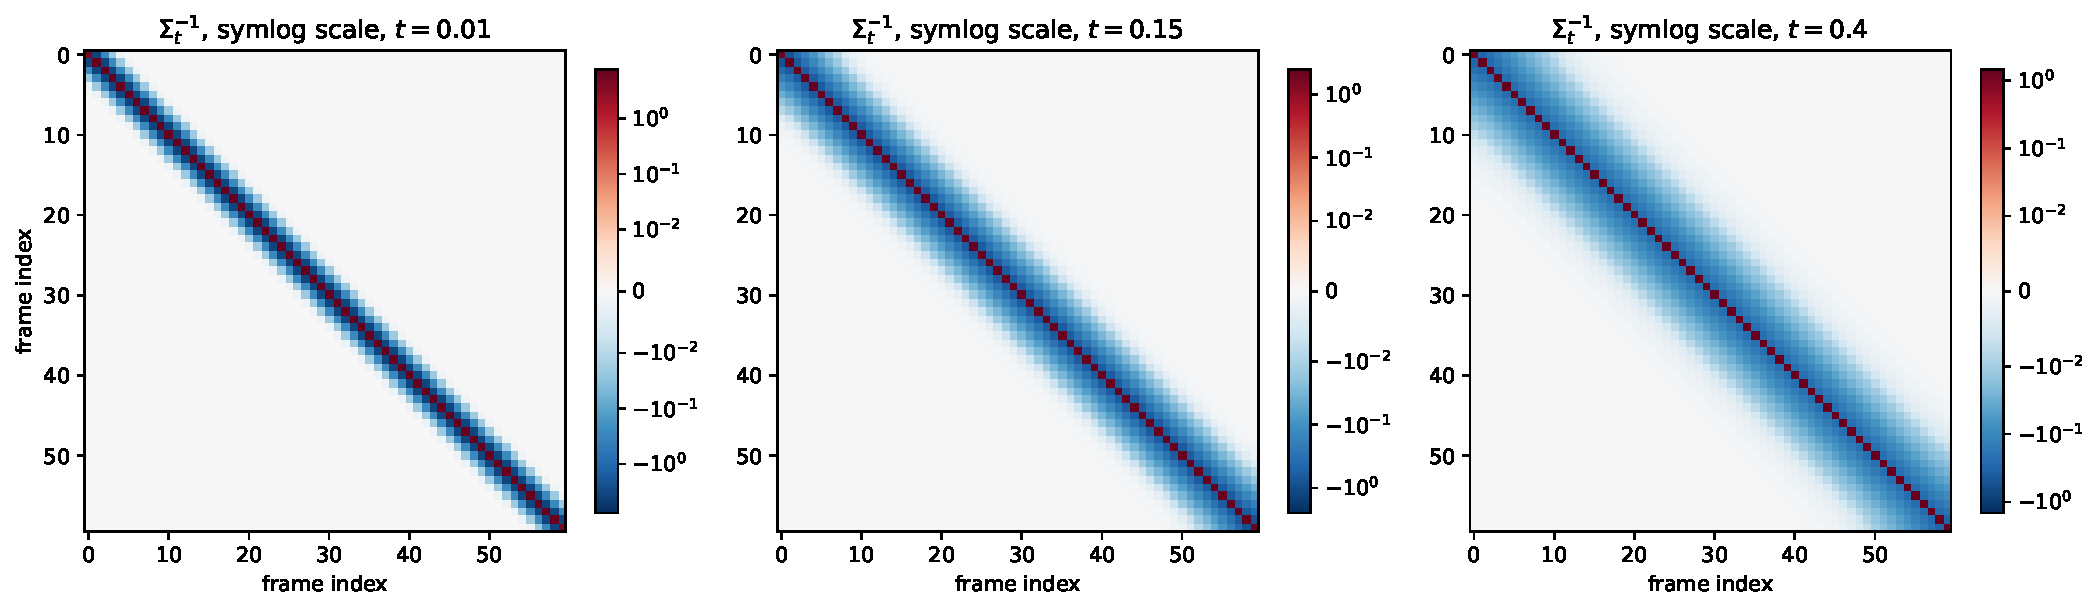
\includegraphics[width=.92\textwidth]{figures/fig08_precision_symlog_heatmaps.pdf}
\caption{Symlog heatmaps of the precision matrix at small and intermediate times. This display makes the weak but exact early-time fill-in visible, addressing the meeting request for a scale that does not wash out small entries.}
\end{figure}

\begin{figure}[H]
\centering

\includegraphics[width=.92\textwidth]{figures/fig04_tridiag_fraction_condition.pdf}
\caption{Left: tridiagonal mass fraction and off-band mass. Right: condition number of $\Sigma_t$. Delocalization and spectral flattening are simultaneous but conceptually different effects.}
\end{figure}

\begin{figure}[H]
\centering

\includegraphics[width=.92\textwidth]{figures/fig05_precision_row_profile.pdf}
\caption{A row profile of the noisy precision. At small times the mass sits on the central site and nearest neighbors; at intermediate times it spreads across the sequence; at large times it contracts back to a diagonal profile.}
\end{figure}

\begin{figure}[H]
\centering
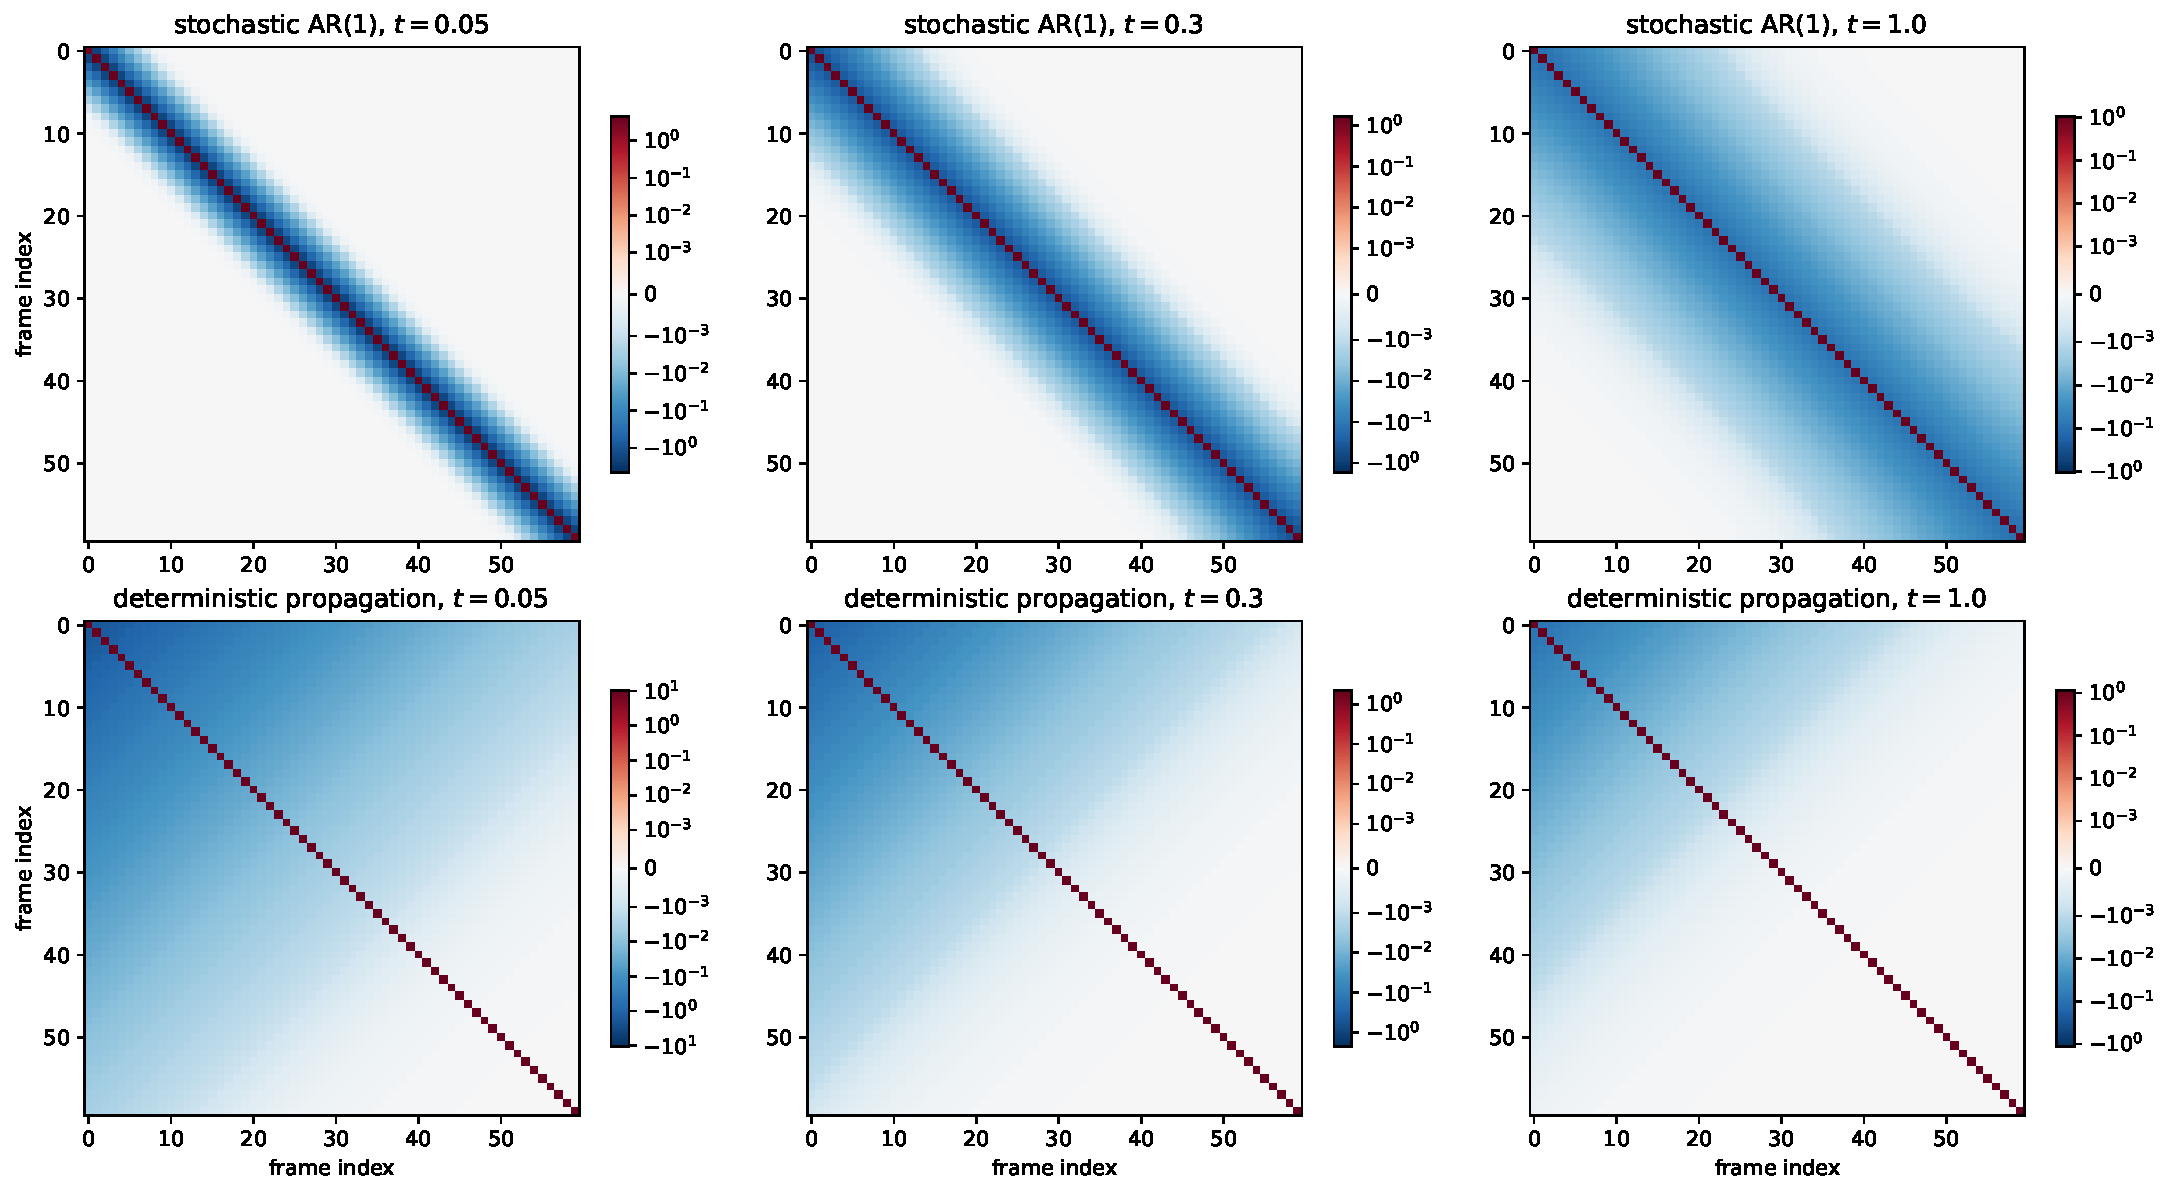
\includegraphics[width=.92\textwidth]{figures/fig09_deterministic_vs_stochastic_precision.pdf}
\caption{Comparison between the stochastic Gaussian AR(1) benchmark and the deterministic-propagation benchmark. The stochastic case starts from a local clean precision; the deterministic case starts from a rank-one clean covariance and immediately exhibits global dense couplings after noising.}
\end{figure}

\begin{figure}[H]
\centering
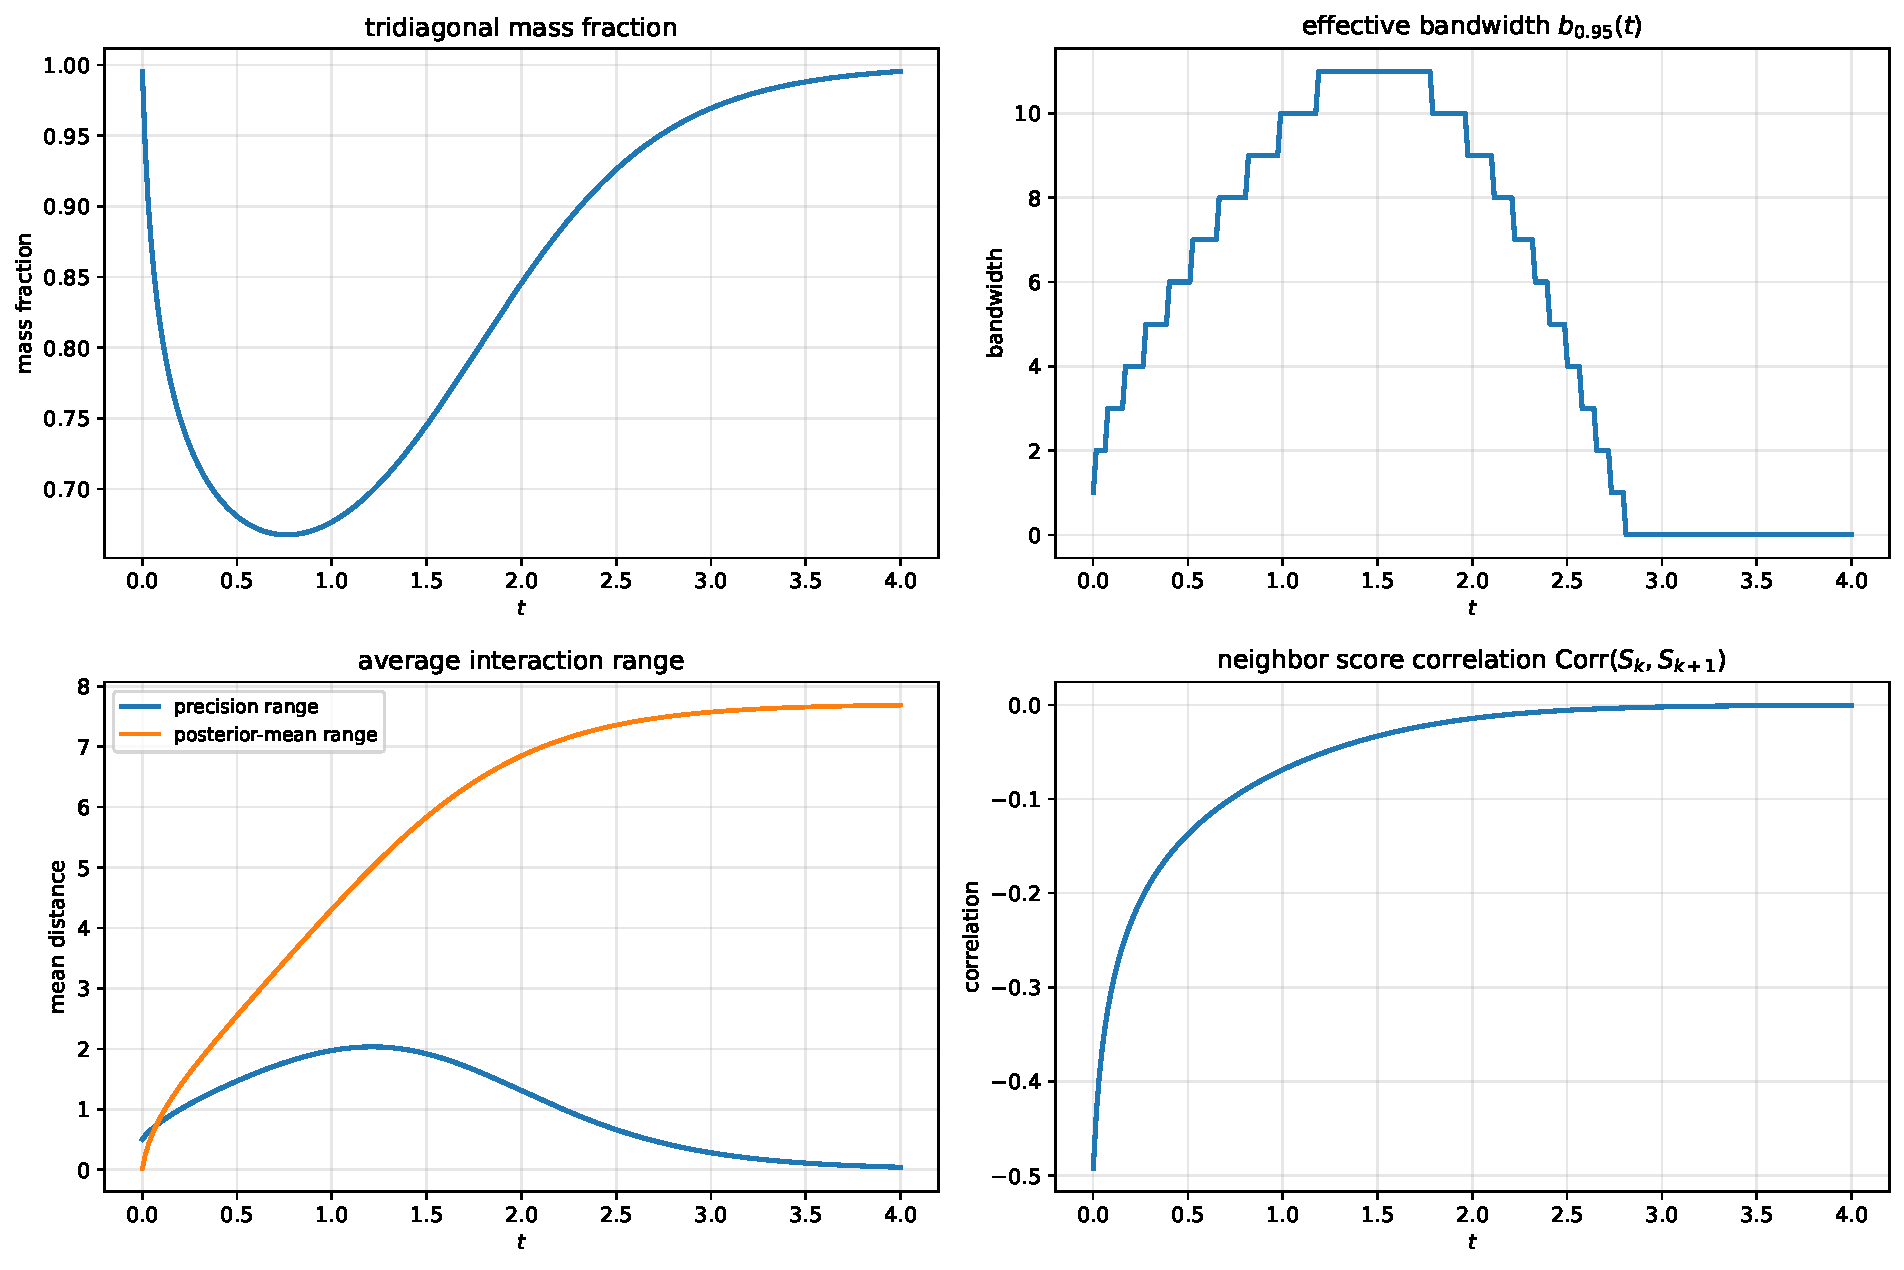
\includegraphics[width=.92\textwidth]{figures/fig10_locality_observables.pdf}
\caption{Locality observables as functions of diffusion time: tridiagonal mass fraction, effective bandwidth, average interaction range, and neighboring-score correlation. These summarize the intermediate regime quantitatively.}
\end{figure}

\begin{figure}[H]
\centering
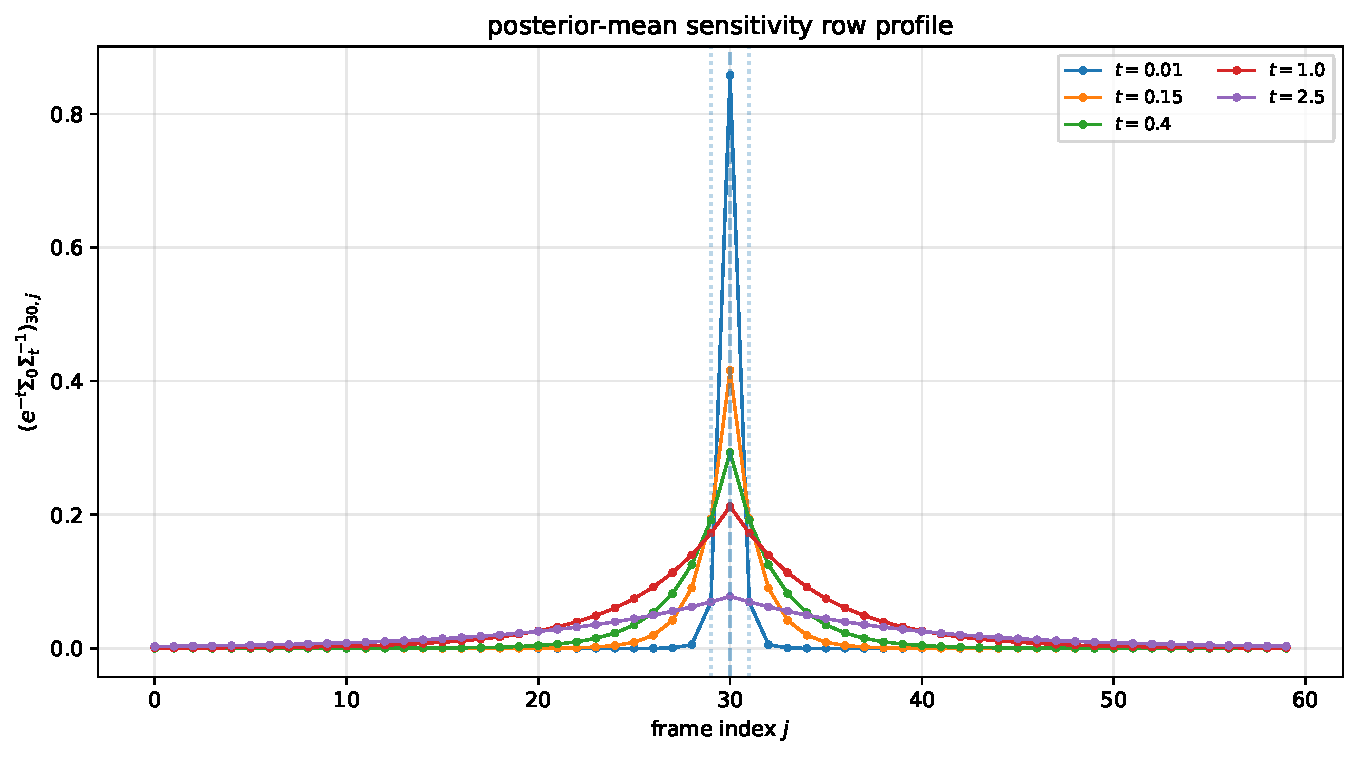
\includegraphics[width=.92\textwidth]{figures/fig11_posterior_mean_profile.pdf}
\caption{Posterior-mean sensitivity profile. This is the matrix $G_t=e^{-t}\Sigma_0Q_t$, which often provides a more intuitive reconstruction-based view of locality than the precision itself.}
\end{figure}

\begin{thebibliography}{99}

\bibitem{draftar1}
G.~Mantovani and M.~Lomel\'e.
\newblock \emph{Joint Score of a Diffusion Model Applied to an AR(1) Sequence: A Self-Contained Derivation}.
\newblock MSc thesis notes, Bocconi University, 2025--2026.

\bibitem{structure}
G.~Mantovani and M.~Lomel\'e.
\newblock \emph{The Structure of $\Sigma_t$ and $\Sigma_t^{-1}$ in the AR(1) Diffusion Model: Explicit Inversion, Spectral Decomposition, and Numerical Study}.
\newblock MSc thesis notes, Bocconi University, March 2026.

\bibitem{anatomy}
G.~Mantovani and M.~Lomel\'e.
\newblock \emph{The Anatomy of $\Sigma_t$ and $\Sigma_t^{-1}$: How Diffusion Noise Reshapes the Score of an AR(1) Sequence}.
\newblock MSc thesis notes, Bocconi University, March 2026.

\bibitem{companion}
G.~Mantovani and M.~Lomel\'e.
\newblock \emph{Mathematical Companion: Deep-Dive Explanations for the $\Sigma_t$ Analysis}.
\newblock MSc thesis notes, Bocconi University, March 2026.

\bibitem{mezardnotes}
M.~M\'ezard.
\newblock \emph{Generative Diffusion Updated Notes}.
\newblock Lecture notes, December 2025.

\bibitem{biroli2023}
G.~Biroli and M.~M\'ezard.
\newblock Generative diffusion in very large dimensions.
\newblock \emph{arXiv preprint arXiv:2306.03518}, 2023.

\bibitem{meetingtranscript}
G.~Mantovani, M.~Lomel\'e, M.~M\'ezard, and J.~Garnier-Brun.
\newblock \emph{Meeting transcript on the AR(1) diffusion benchmark and next research directions}.
\newblock Working transcript, March 2026.

\end{thebibliography}


\end{document}
